\chapter{Bitácora}

\begin{itemize}
    \item 11OCT22: Reu en Navales. jviu, pang, victor, carlos: 
    \begin{itemize}
        \item 
    aprendemos a usar latex
        \item Hablamos sobre la web git de pyexams \cite{pyexamsgit}
        \item Miramos texsurgery, sus test unitarios, etc
        \item Carlos recomienda que hablemos del propósito de pyexams.
    \end{itemize}
    \begin{itemize}
        \item Instala texsurgery, corre todos los tests, tb los de la doc., documenta los problemas que surjan...
        \item Pedimos permiso para overleaf para carlos 
    \end{itemize}
    \item Semana 11OCT-18OCT
    \begin{itemize}
        \item Instalado texsurgery y ejecutado pruebas unitarias
        \item Instalado pyexams y ejecutado ejemplos python/en y /python/es, 'es' funciona sin error, 'en' falla 
    \end{itemize}
    \item 18OCT22: Reu en Navales. jviu, pang, victor:
    \begin{itemize}
        \item Trabajo simultáneo con overleaf
        \item Juan manda deberes para aprender LaTeX: crear un examen
        \item Comprobamos que tras instalar pyexams algún ejemplo falla por no tener instalados todos los paquetes texlive
    \end{itemize}
    \item Semanas 18OCT-02NOV
    \begin{itemize}
        \item TODO: Documentar estado de texsurgery y pyexams, primeras impresiones, en capítulo estadocuestion
        \item TODO: Aprender latex con el manual de wikibooks
        \item TODO: examen de prueba
        \begin{enumerate}
            \item Me he basado en los \href{https://framagit.org/pang/pyexams/-/tree/master/examples}{ejemplos de exámenes de pyexams}, para generar el examen de ejemplo proporcionado.
            \item Escrito la versión 1 del examen en LaTeX.
            \item Transformado el documento para que la ejecución con pyexams genere las dos versiones del examen
            \item Ejecutado con pyexams con los siguientes resultados
            \begin{enumerate}
                \item Error por encoding, el fichero utilizado tenia un encoding distinto a UTF-8, cambiado el encoding a UTF-8 con el editor de texto.
                \item Error por formato de las sentencias sif, corregido.
                \item Ejecutado sin errores en la terminal, pero no he declarado bien las partes de ejercicio y de solución para pyexams (sale tanto el ejercicio como la solución en ambos).
                \item Declarado la pregunta y la solución dentro del fichero tex, ahora el enunciado se genera correctamente pero la solución no. El pdf de solución tiene la primera página en blanco (solo con la cabecera) y la solución se corta en la segunda pagina.
            \end{enumerate}
        \end{enumerate}
        \item TODO: Averiguar/Documentar los paquetes texlive que hay que instalar para que los ejemplos de pyexams funcionen.
        \item TODO: \url{https://framagit.org/pang/pyexams/-/issues/5} \\
        Añadir un argumento extra para el archivo \textit{students.csv} en el envío de correos.
        \begin{itemize}
            \item Primero he querido probar el funcionamiento del envio de correos, utilizando las \href{https://framagit.org/pang/pyexams/-/tree/master/examples}{plantillas de ejemplo de pyexams}.
            \begin{itemize}
                \item Al poner el envío con mi correo de la universidad me daba un problema del servidor SSL, probablemente he puesto el puerto mal. He utilizado un correo de gmail para el envío, y he tenido que crear una contraseña de aplicación por la configuración de seguridad de google.
                \item Ha dado un error al no existir el fichero pdf que enviar. La opción \textit{send} necesita que generes primero el examen.
            \end{itemize}
            \item Los argumentos que recibe pyexams se tratan con la librería python \textit{argparse}, así que he mirado la documentación de esta librería y los otros argumentos de pyexams para crear el nuevo argumento
            \begin{itemize}
                \item Añadido un nuevo argumento (-sf fichero.csv) que recibe el nombre del fichero, con valor por defecto \textit{students.csv}.
                \item Probado el funcionamiento de tanto el nuevo argumento como el envio normal por defecto.
            \end{itemize}
        \end{itemize}
        \item TODO: Resuelve \url{https://framagit.org/pang/pyexams/-/issues/2}
        \begin{enumerate}
            \item Mira en texsurgery cómo se copia texsurgery.sty a la carpeta de trabajo: \url{https://framagit.org/pang/texsurgery/-/commit/6d4e05950f953a1ff8932a058c5421b6dd8924bb}
            \begin{itemize}
                \item En \textit{setup.py}: \textit{include\_package\_data=True} e incluye el paquete con los datos
                \item En \textit{command\_line.py}: comprueba el argumento y copia el fichero con \textit{shutil.copy()}. Obtiene la ubicación del fichero a partir de \textit{texsurgery.\_\_path\_\_[0]}.
            \end{itemize}
            \item Mira en \url{https://framagit.org/pang/pyexams/-/blob/master/pyexams/command_line.py} cómo se añaden opciones a la línea de comandos
            \item Prepara una plantilla para un examen básico, o para un envío de emails básico
            \begin{itemize}
                \item plantilla de examen en latex
                \item plantilla de configuración de correo (hay una en examples)
                \item plantilla de correo a enviar (hay una en examples)
            \end{itemize}
            \item une la línea de puntos
            \item piensa cómo hacerlo con plantillas por lo menos en castellano e inglés
        \end{enumerate}
    \end{itemize}
    \item 02NOV22: Reu en Navales. pang:
    \begin{itemize}
        \item Arreglado el error por el que generaba la solución en una sola página, con \href{https://project.auto-multiple-choice.net/boards/2/topics/9759?r=9819#message-9819}%
        {la solución de Auto Multiple Choice}. Sustituye el entorno \textit{question} por un nuevo comando. Este comando comprueba una variable de AMC e imprime la solución cuando debe.
        \item Issue 5:
        \begin{enumerate}
            \item Cambiado el argumento para almacenarlo en formato \textit{string} en vez de \textit{List}.
            \item Configurado la clave SSH para framagit.
            \item Subido la solución a una nueva rama del repositorio: \textit{issue5}
        \end{enumerate}
    \end{itemize}
    \item Semana 02NOV-08NOV
    \begin{itemize}
        \item Cerrar el issue 5
        \item Continuar el trabajo
    \end{itemize}
    \item 08NOV22: Reu en Navales. pang:
    \begin{itemize}
        \item TODO: crear issue con la opción de generar a LateX, en vez de generar pdf. Basta con no borrar el tex que ya generamos (cuando hay error no se borra, de hecho).
        \begin{itemize}
            \item Creado el \href{https://framagit.org/pang/pyexams/-/issues/7}{Issue 7}
        \end{itemize}
        \item Pensamos si pandoc puede ayudar a convertir a jupyter ipynb, pero también dudamos si este issue puede interesar al público en general.
        \item Pensar: escanear exámenes. Puede ser útil \url{https://stackoverflow.com/questions/22898145/how-to-extract-text-and-text-coordinates-from-a-pdf-file} (pang conocía \url{https://pypi.org/project/PyPDF2/} pero no parece que sirva para sacar las coordenadas del formulario, sólo los campos). también puede ayudar mirar el código de R-exams: \url{https://cran.r-project.org/web/packages/exams/index.html}. En la siguiente reunión (22NOV), pang intentará detaller los pasos y/o invitar a más gente. Después de esa reu, deberíamos quedar con Sandra.
    \end{itemize}
    \item Semanas 08NOV-22NOV
    \begin{itemize}
        \item Escanear exámenes
        \begin{itemize}
            \item Id de alumno: cuadros del encabezado
            \item Lectura del examen: varias páginas, formato (pdf, jpg, ...)
            \item Para cada ejercicio:
            \begin{itemize}
                \item \# de ejercicio dentro del examen
                \item identificar los cuadros y sus posiciones (OpenCV 
                \href{https://towardsdatascience.com/checkbox-table-cell-detection-using-opencv-python-332c57d25171}{1}, 
                \href{https://stackoverflow.com/questions/55763858/how-to-detect-and-find-checkboxes-in-a-form-using-python-opencv}{2}, 
                \href{https://www.fuzzylabs.ai/blog-post/checkbox-detection-with-opencv}{3}, 
                \href{https://loichau997.medium.com/apply-computer-vision-on-the-questionaire-image-to-detect-ticked-checkboxes-646e9245d293}{4}; 
                paquete \href{https://pypi.org/project/boxdetect/}{boxdetect})
                \item cuadros marcados
            \end{itemize}
            \item obtener la solución
            \begin{itemize}
                \item según el id del alumno
                \item a partir del pdf con la solución (detectando las cajas como con el escaneado, pero posiciones distintas ya q puede tener explicación)
                \item a partir de otro archivo q generar: pdf solución simplificado (que tenga las mismas posiciones que el enunciado, simplificaría el escaneo), o txt con datos sencillos (p.ej: \# de alumno, \# de ejercicios, \# numero de cuadros, \# cuadro solucion)
            \end{itemize}
        \end{itemize}
    \end{itemize}
    \item 22NOV22: Reu en Navales. pang, :
    \begin{itemize}
        \item TODO: Estudiar como obtener la informacion de pdfminer: casillas, tags y coordenadas
        \item TODO: definir modulos para escanear examenes, inputs/outputs
    \end{itemize}
    \item 25NOV22: Reu en Teams. pang, sandra:
    \begin{itemize}
        \item Definir distintos tipos de preguntas que acepta pyexams
        \item Diagrama de componentes/clases
        \item Lista de requisitos -> Hacer una entrevista de requisitos en navales
        \item Metodologias Agiles -> sacar de la Bitacora y la lista de requisitos los sprints
        \item Definir los conocimientos utilizados para la realizacion del TFG y de donde se ha obtenido 
        \item Documentar mejor las pruebas realizadas con imágenes
        \item Utilización de cuadernos jupyter para la realización de pruebas
    \end{itemize}
    \item Semana 22NOV-29NOV
    \begin{itemize}
        \item Creado un diagrama inicial de los modulos de Escanear Examenes (en IdeasSueltas)
        \item Probado en un cuaderno jupyter tanto los visitors de pyPDF2 como la libreria boxdetect
    \end{itemize}
    \item 29NOV22: Reu en Navales. pang:
    \begin{itemize}
        \item Cambiando pyPDF2 en constantes - FieldDict Attributes Rect consigue los rectangulos (correo).
        \item TODO comparar las coordenadas de pyPDF2 y boxdetect
    \end{itemize}
    \item Semanas 29NOV-13DIC
    \begin{itemize}
        \item Realizado los cambios de pang a PyPDF2 en local
        \item Comparado las coordenadas de las casillas en PyPDF2 y boxdetect
        \begin{figure}
            \centering
            \begin{minipage}{.5\textwidth}
                \centering
                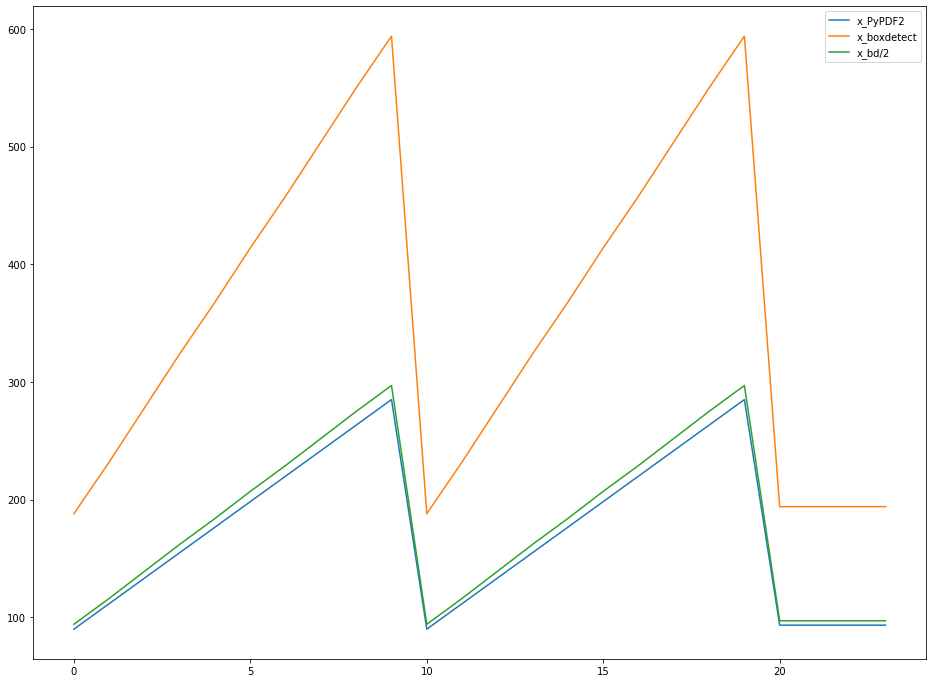
\includegraphics[width=0.9\textwidth]{figures/graph_x.png}
                \caption{Comparación de las coordenadas x}
                \label{fig:graph_x}
            \end{minipage}%
            \begin{minipage}{.5\textwidth}
                \centering
                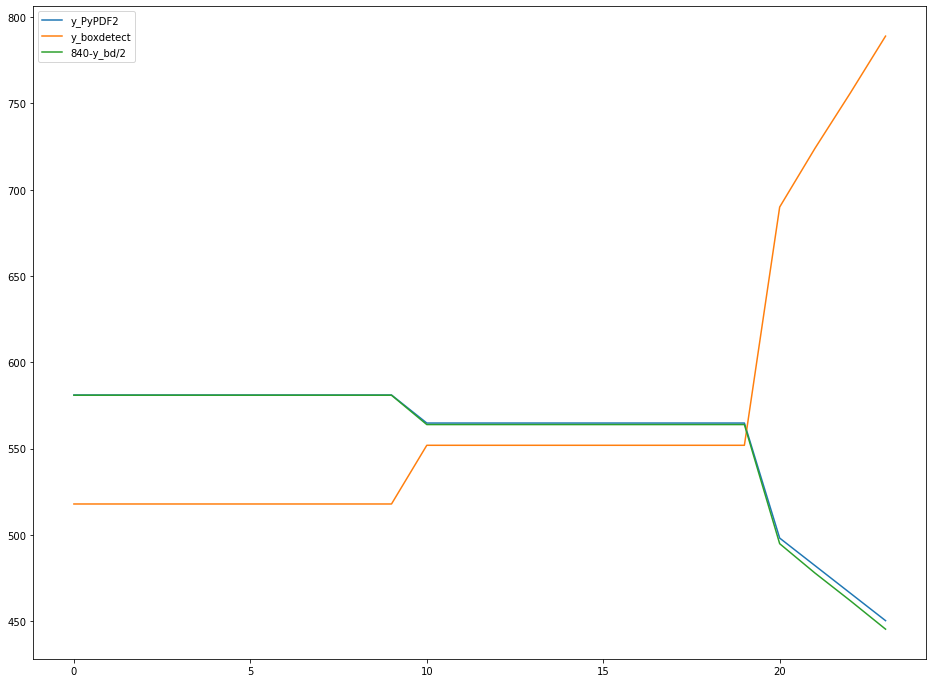
\includegraphics[width=0.9\textwidth]{figures/graph_y.png}
                \caption{Comparación de las coordenadas y}
                \label{fig:graph_y}
            \end{minipage}
        \end{figure}
        \\ Las coordenadas parecen estar escaladas 1:2, y la coordenada y esta invertida
        \item Generado exámenes escaneados para probar la detección de casillas (Ideas Sueltas)
        \item 
    \end{itemize}
    \item 13DIC22: Reu en Navales:
    \begin{itemize}
        \item En mi ordenador no genera las casillas binarias con identificadores correctos, estudiar posibilidad de utilizar codigos qr (pang) con la informacion (examen, copia, num pagina) en formato JSON
        \item Uso de los puntos de las esquinas para corregir la perspectiva (perspective correction)
        \item Definido 'escanear examenes' en 3 funciones:
        \begin{itemize}
            \item Detect: 'detectar diseño', obtiene de los pdfs solucion generados las coordenadas de cada casilla, el estado correcto y los datos del alumno; que extrae a un fichero json
            \item Analyse: en el fichero pdf con los examenes escaneados, identificar cada examen, pagina, ejercicio y casilla a partir de los identificadores (puntos de las esquinas, casillas binarias, codigo qr) y las coordenadas de las casillas; extraer tambien a json
            \item Match: a partir de las salidas de las otras dos funciones, puntuar cada ejercicio
        \end{itemize}
        \item Division del problema en capas: Grupo > Examen > Papel > Pregunta > Casilla
        \item Diagramas de tareas/etapas/flujos (posibilidad de omitir etapas segun los flujos: grade en caso de encuestas)
    \end{itemize}
    \item Semana 13DIC-20DIC
    \item Diseño de prototipo de función "Escanear exámenes", TODO:
    \begin{itemize}
        \item TODO: Detectar diseño
        \begin{itemize}
            \item Leer alumnos.csv y de ahi obtener cada fichero pdf de solucion
            \item Leer de (el fichero tex / los pdf de solucion) el numero y nombre de ejercicios y el numero de casillas
            \item Obtener de los pdf de solucion las casillas, sus coordenadas y estado (on/off)
            \item Exportar los datos a JSON
        \end{itemize}
        \item TODO: Analizar escaneo
        \begin{itemize}
            \item Leer el pdf con los examenes escaneados pagina a pagina
            \item Obtener la informacion de cada pagina (examen, copia y num pagina)
            \item Identificar las casillas y sus estados
            \item Exportar los datos a JSON
        \end{itemize}
        \item TODO: Match
        \begin{itemize}
            \item Obtener la informacion de los JSON de detect y analyse
            \item Puntuar cada examen
        \end{itemize}
    \end{itemize}
    \item Diseño de prototipo de función "Escanear exámenes", pruebas realizadas:
    \begin{itemize}
        \item "t\_json.ipynb": pruebas del formato de datos a guardar en JSON y de la lectura y escritura de estos datos.
        \item "t\_pdftopng.ipynb": ya que para identificar las casillas con cv2 se trabaja con ficheros png, hay q transformar los ficheros pdf en 1/varios pngs. Para esta transformación pruebo con la librería pdf2image. También contiene una prueba de identificar casillas de pngs mediante cv2.
        \item "t\_scan.ipynb": prototipo de la función "Escanear exámenes", con funciones \textit{detect}, \textit{analyse} y \textit{match}.
        \item "checkboxes.py": funciones utilizadas en el prototipo: \textit{find\_checkboxes}, \textit{check\_marcked} y \textit{match}.
    \end{itemize}
    \item 20DIC22: Reu en Navales:
    \begin{itemize}
        \item Dividir por capas la función "Escanear exámenes":
        \begin{itemize}
            \item Examen: considerando un mismo examen generado con pyexams a partir de un fichero tex
            \item Variante: para cada una de las variantes generadas con pyexams, con distintas soluciones
            \item Alumno*: para los distintos estudiantes que realicen una misma variante (*¿Como identificar el examen de cada alumno?)
            \item Ejercicios: identificar los ejercicios y sus casillas, para detectar el patrón del examen y la solución, utilizar dicho patrón para detectar las casillas en el examen escaneado y comprobar con la solución.
            \item Casillas: detectar las casillas, sus coordenadas y si están marcadas
        \end{itemize}
        \item Añadir QR a examenes desde pyexams:
        \begin{itemize}
            \item Librería \href{https://ctan.org/pkg/qrcode?lang=en}{qrcode} de latex 
            \item Añadir funcionalidad a pyexams para insertar un codigo qr, haciendo uso de la libreria qrcode, en el lugar indicado con '\textbackslash{}QR': '\textit{replace(\textbackslash{}QR, JSON)}'
        \end{itemize}
    \end{itemize}
    \item 20DIC22-20ENE23
    \begin{itemize}
        \item Definición de la función 'Escanear examen'
        \begin{itemize}
            \item Dividido la función en 4 funciones que actúan en distintas capas:
            \begin{figure}
                \centering
                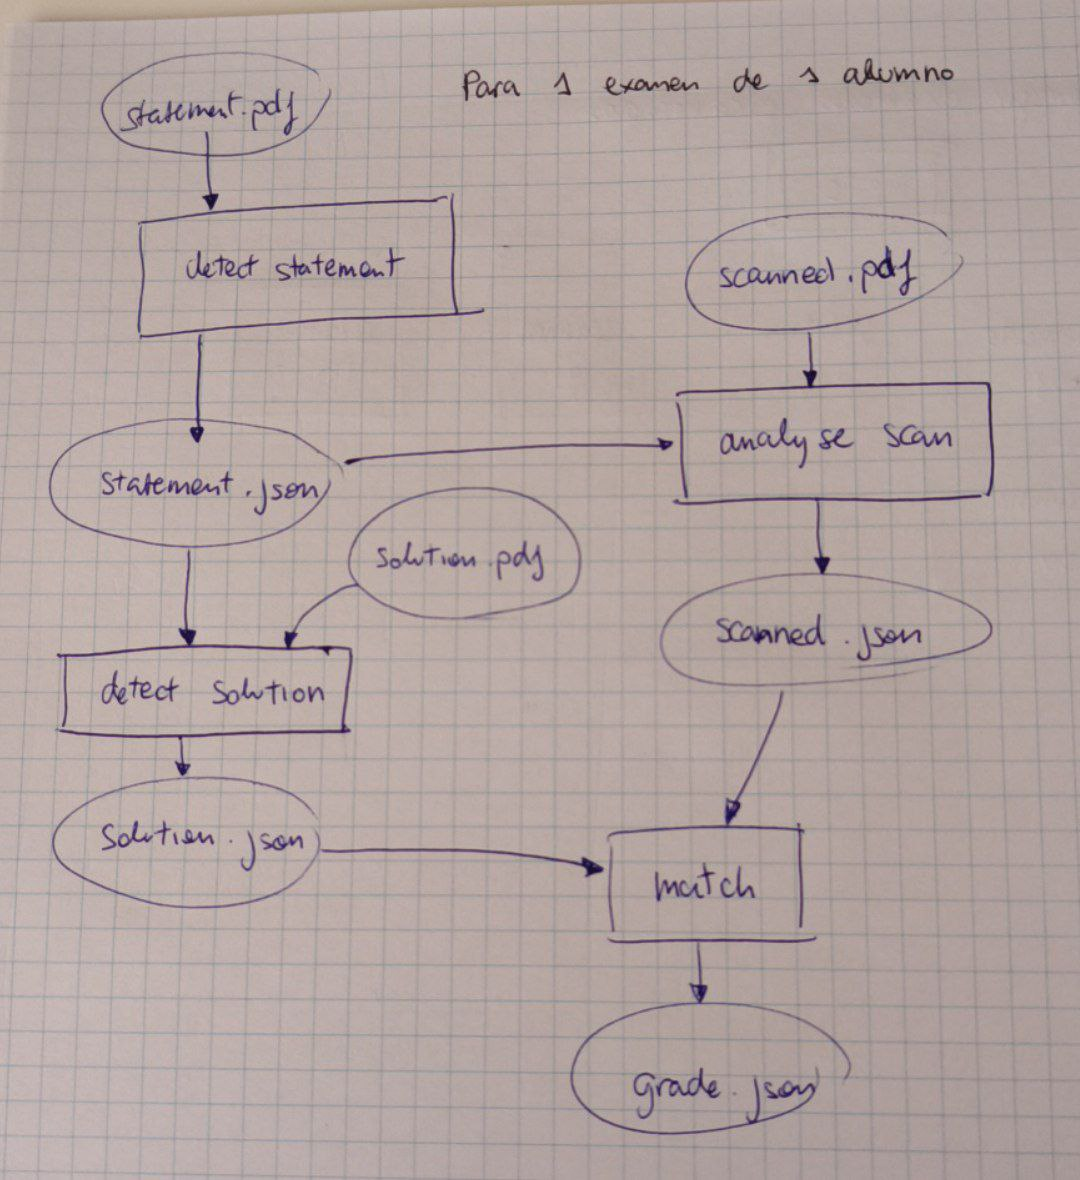
\includegraphics[width=0.8\textwidth]{figures/diag_comp_1ex.jpeg}
                \caption{Diagrama de componentes de la función Escanear Exámenes}
                \label{fig:diagramaComp}
            \end{figure}
                \item Detect Statement: obtiene de un fichero pdf generado por pyexams el diseño del examen: sus ejercicios y las casillas de cada ejercicio, junto a las coordenadas de las casillas. Esta función actúa en la capa de examen, ya que en teoría las variantes de los exámenes no modifican la posición de las casillas (*las variantes podrían tener distintas coordenadas, pero no debería ser un problema). Guarda los datos obtenidos en un fichero JSON
                \item Detect Solution: obtiene de un fichero pdf generado por pyexams las casillas marcadas en cada ejercicio en la solución del examen. Esta función actúa en la capa de variante, ya que la solución de cada variante es diferente. Guarda los datos en un fichero JSON que genera a partir del generado en detect statement.
                \begin{figure}
                    \centering
                    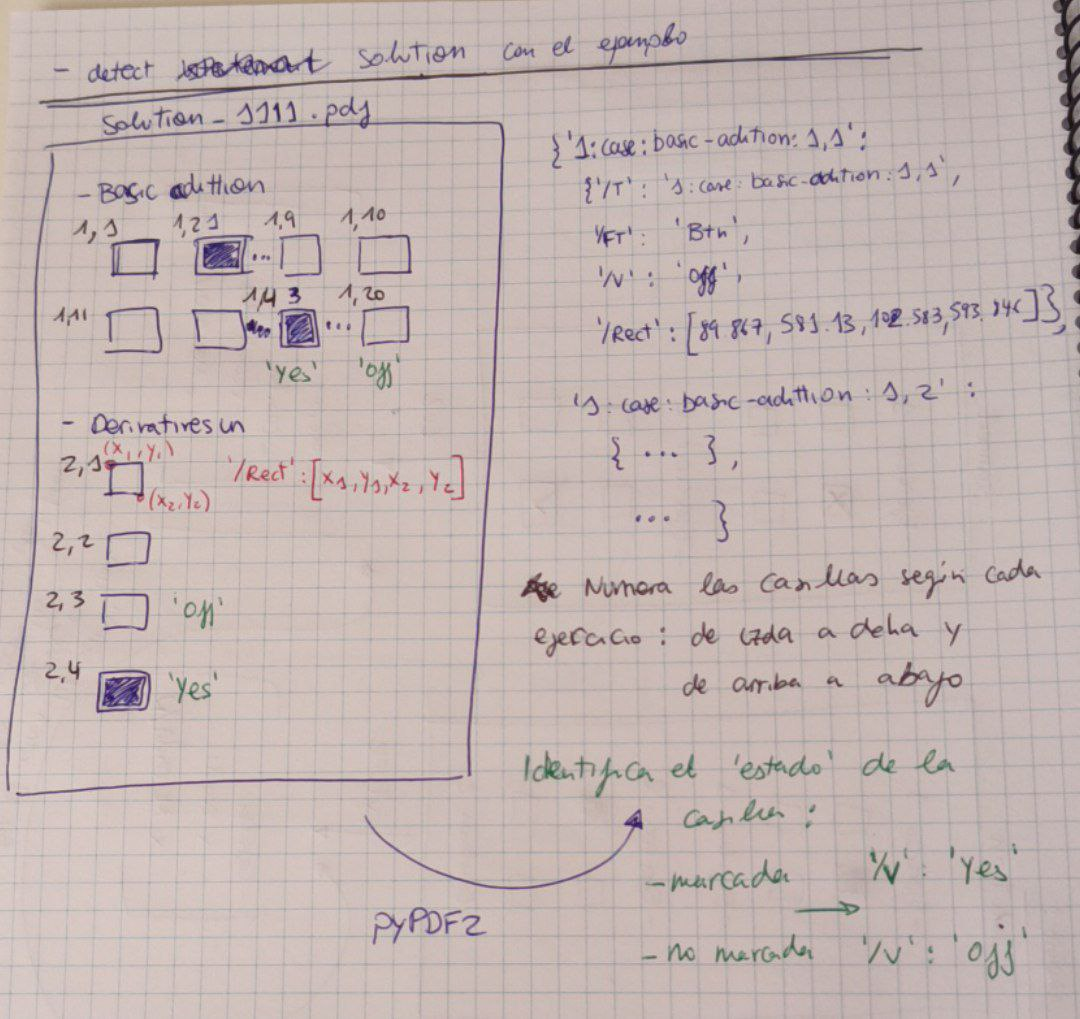
\includegraphics[width=0.8\textwidth]{figures/detect_sol.jpeg}
                    \caption{Ejemplo de Detect Solution}
                    \label{fig:exDetectSol}
                \end{figure}
                \item Analyse Scan: obtiene de un fichero pdf con el examen 'escaneado' realizado por un alumno: las casillas de cada ejercicio y si están marcadas. Para detectar las casillas hacen falta obtener imágenes de cada pagina, por lo que primero genera estas. Detecta las casillas y sus coordenadas con OpenCV, además de su estado (si están marcadas o no). Compara las casillas leídas con la estructura obtenida en detect statement, y guarda la información de qué casillas hay marcadas. Funciona en la capa de alumno. Guarda la información de las casillas marcadas en un JSON modificando el generado en detect statement
                \begin{figure}
                    \centering
                    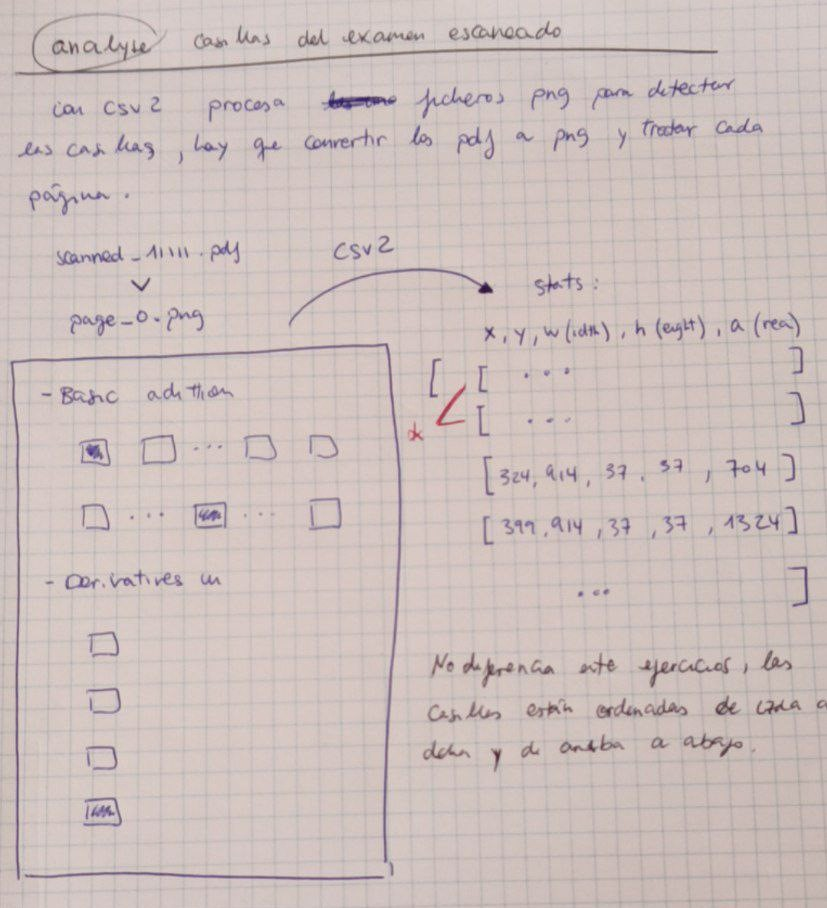
\includegraphics[width=0.8\textwidth]{figures/analyse_scan.jpeg}
                    \caption{Ejemplo de Analyse Scan}
                    \label{fig:exAnalyseScan}
                \end{figure}
                \item Match: Compara los ficheros JSON generados en detect solution y analyse scan para valorar la puntuación del examen. 
        \end{itemize}
        \item Prototipo de Escanear exámenes
        \begin{itemize}
            \item Esquema de funcionamiento: figura \ref{fig:protEscExam}
                \begin{figure}
                    \centering
                    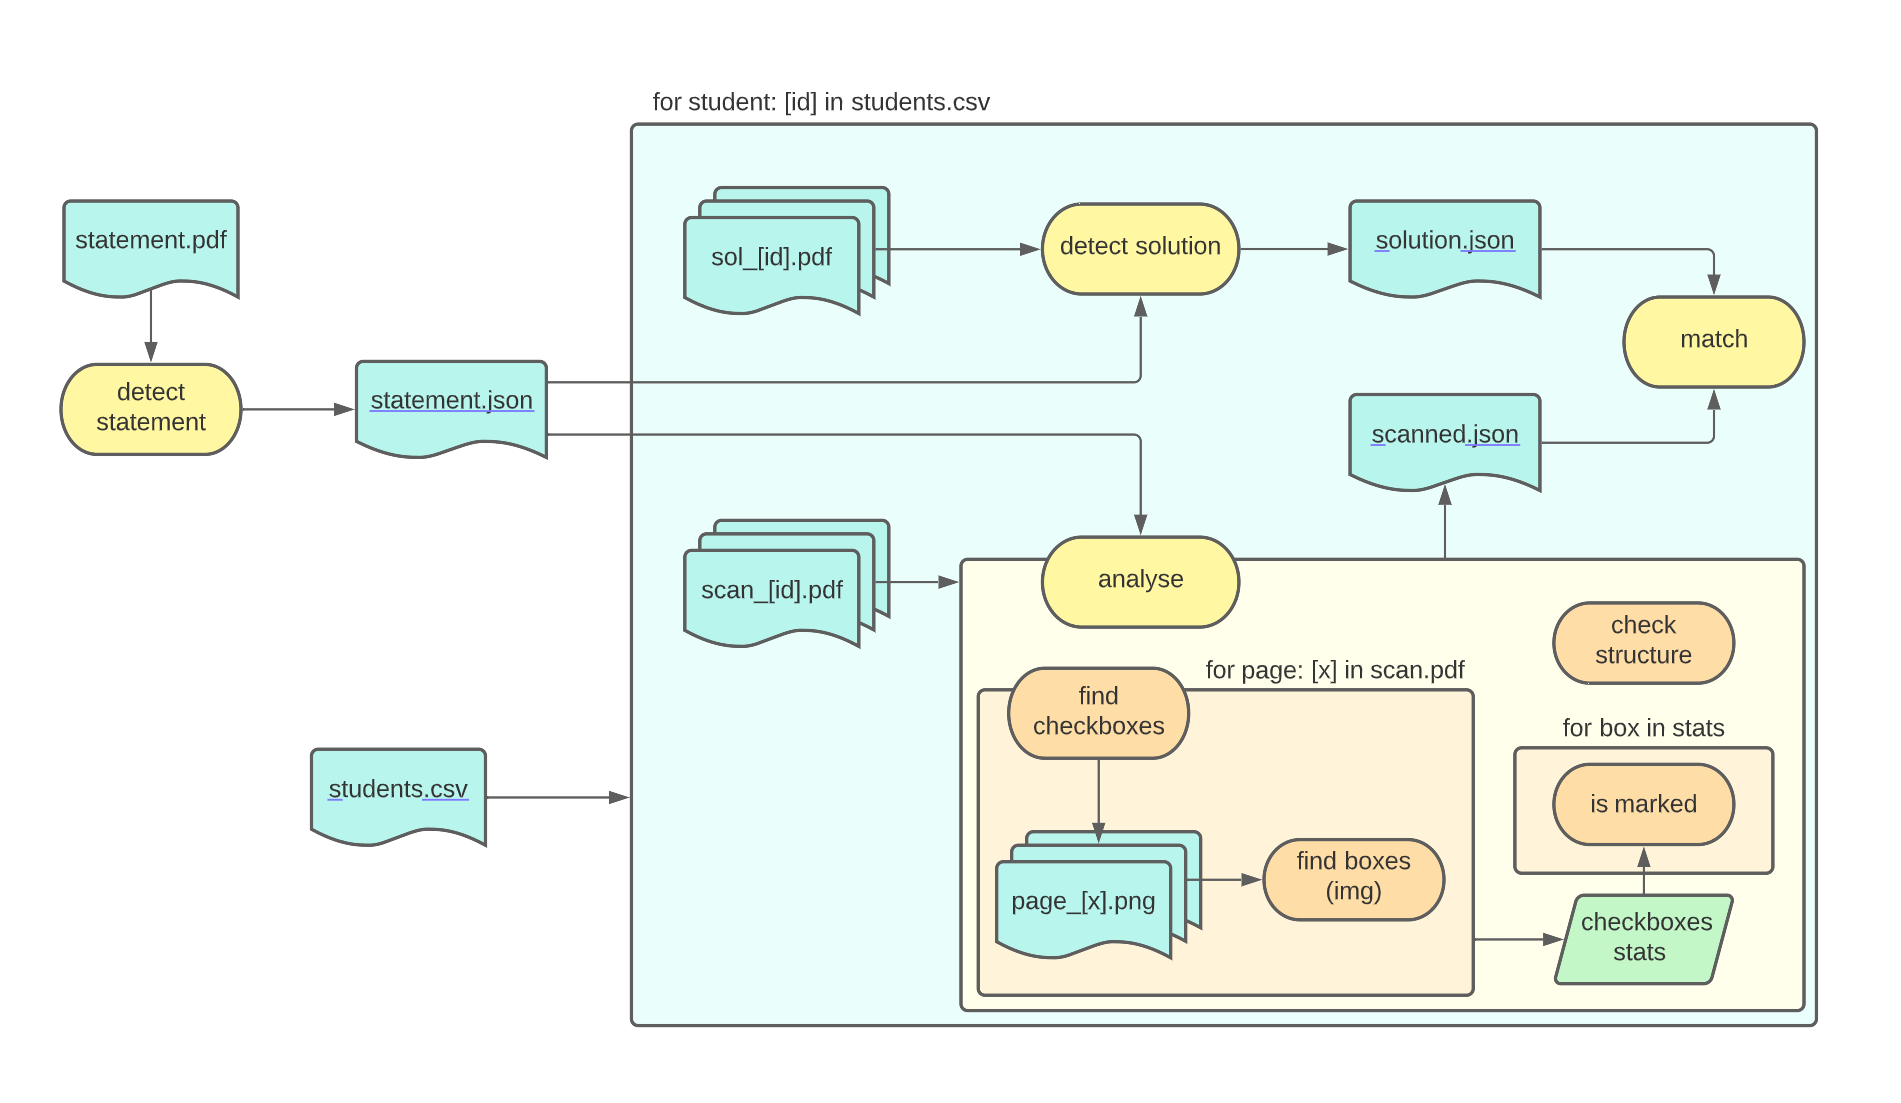
\includegraphics[width=\textwidth]{figures/esquema_prototipo.png}
                    \caption{Esquema del prototipo de Escanear exámenes}
                    \label{fig:protEscExam}
                \end{figure}
                \begin{itemize}
                    \item Detect statement: lee un único enunciado del examen y genera un json con la estructura de este: ejercicios, casillas y coordenadas de estas. Utiliza la versión modificada de pyPDF2 para detectar las casillas.
                    \item Para cada alumno en students.csv:
                    \begin{enumerate}
                        \item Detect solution: lee la solución de la variante, comprueba que la estructura es igual a la del enunciado y guarda tanto la estructura como las casillas que están marcadas en un json. Utiliza la versión modificada de pyPDF2 para detectar las casillas.
                        \item Analyse: lee el examen rellenado por el alumno, comprueba que la estructura es igual a la del enunciado y guarda tanto la estructura como las casillas que están marcadas en un json. Utiliza OpenCV para detectar las casillas, en las siguientes funciones:
                        \begin{enumerate}
                            \item Find checkboxes: la forma de detectar las casillas con OpenCV utiliza de entrada un fichero png, así que esta función convierte cada pagina del pdf a un png y detecta las casillas en cada pagina.
                            \item Is marked: la información que extrae OpenCV sobre las casillas, que se puede ver en la figura \ref{fig:casillasCV2}, incluye información de sus coordenadas (x e y), tamaño (ancho y altura) y área interior a la casilla. Este área parece ser mucho menor en las casillas marcadas, así que la función compara este parámetro con el área del rectángulo (ancho por altura) y considera que la casilla está marcada si el parámetro es menor al 80\% del área del rectángulo.
                            \begin{figure}
                                \centering
                                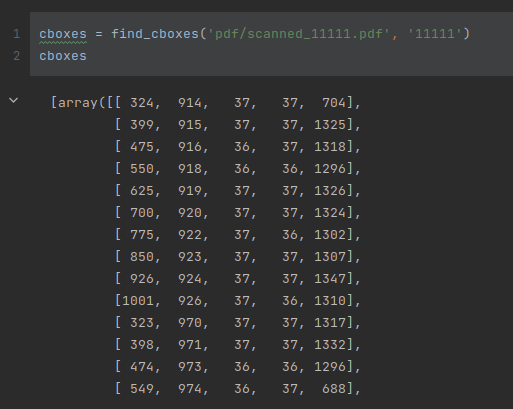
\includegraphics[width=0.7\textwidth]{figures/scan_OpenCV.png}
                                \caption{Información de las casillas obtenida con OpenCV}
                                \label{fig:casillasCV2}
                            \end{figure}
                        \end{enumerate}
                        \item Match: compara los json de solucion y escaneado y devuelve el numero de ejercicios 'bien' (con las mismas casillas marcadas) y el total de ejercicios
                    \end{enumerate}
                \end{itemize}
                \item Cuaderno ipython del prototipo:
        \end{itemize}
    \end{itemize}
    
    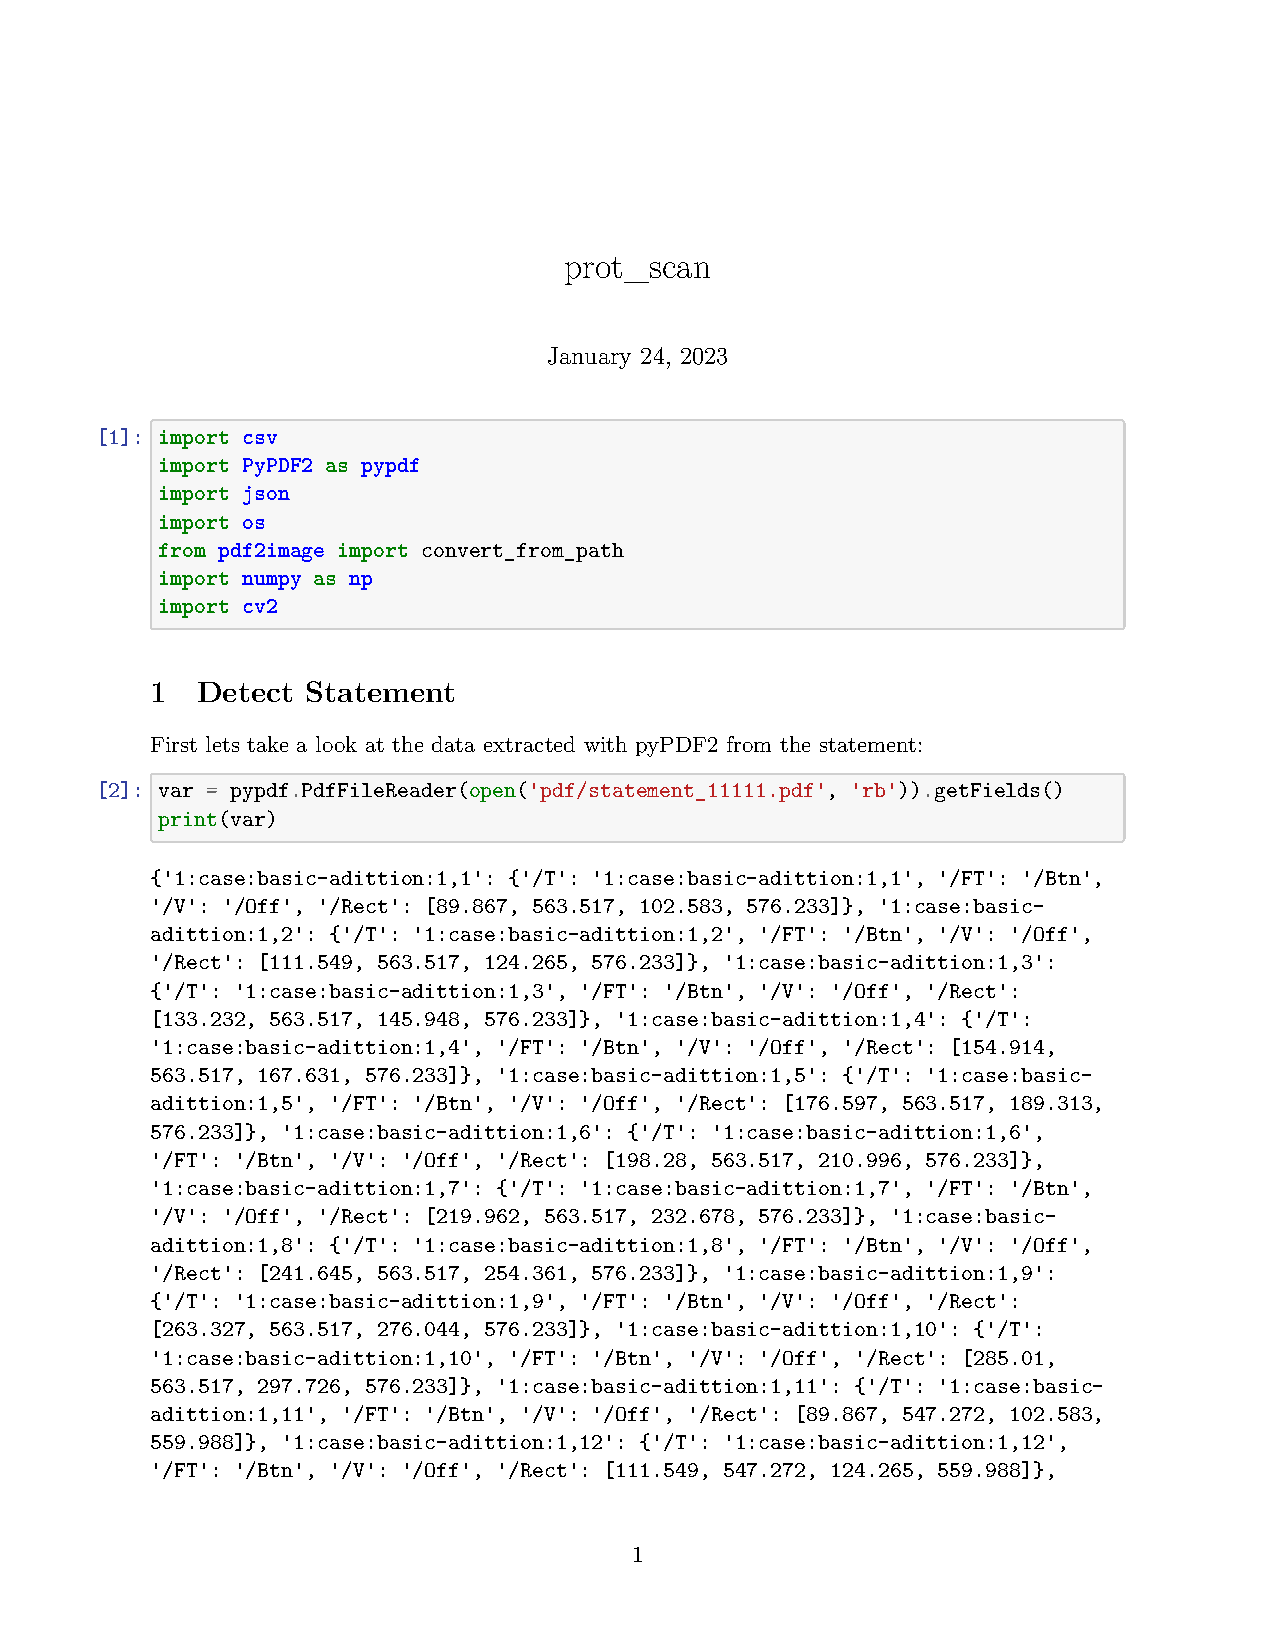
\includepdf[pages=-]{pruebas/prot_scan.pdf}
    
    \item 20ENE23: Reu en Teams:
    \begin{itemize}
        \item TODO: Añadir la funcionalidad de escanear exámenes a pyexams:
        \begin{itemize}
            \item Generar los json de statement/solution al compilar el tex
            \item Funcion scan: "pyexams -scan ruta [fich.json]"
            \begin{itemize}
                \item ruta: si es un pdf, analizar cada examen que se encuentre en el pdf. Si es un directorio, analizar cada pdf dentro de este
                \item fich.json: identifica cada alumno con una variante de examen?
            \end{itemize}
        \end{itemize}
        \item TODO: funcionalidad QR: añadir comando \textbackslash{QR} que pyexams reemplace por un código QR (libreria \href{https://ctan.org/pkg/qrcode}{qrcode} de latex) con datos del examen: [numero de pagina,] variante, id del examen, etc.
        \item TODO: hablar con los de pyPDF2 para incluir los cambios. También: instrucciones de instalación con pyPDF2 modificado
        \item TODO: Analyse alternativo para pdfs rellenados con editor/no escaneados. Realizar primero una busqueda de casillas con pyPDF2, y si no encuentra las casillas buscar con OpenCV.
        \item TEST: pruebas mas extensas de escanear examenes: examen de más páginas, función shuffle, etc..
        \item TEST: probar distintas formas de rellenar casillas: opaca, cruz, tick, etc..
        \item TODO: guardar la información de página en analyse (¿cómo identifica distintas paginas pyPDF?)
        \item TODO: Transformar las paginas escaneadas antes de analizar con OpenCV para rectificar (transformación del qr, puntos de las esquinas de AMC)
        \item TODO: guardar las coordenadas [de solucion y] de escaneado en el json
        \item TODO: funcion match, informacion a guardar en el JSON: para cada ejercicio guardar id, casillas en solucion y en escaneado, y si esta bien
        \item {[}TODO: guardar en .pyexams información de los proyectos ejecutados en el PC{]}
    \end{itemize}
    \item 24ENE23: Reu en Navales
    \begin{itemize}
        \item connected with stats de cv2 parece no detectar cuadrados enteros como casillas
        \item sacar los dpi y min\_width de las funciones de escanear examenes para que sean variables, y obtenerlos en funcion del pdf
        \item trabajo futuro descrito en el correo de pablo tras reunion teams 
        \item generar un qr en cada cara, si se usa para corregir ángulo
        \item click derecho en un archivo para corregir
    \end{itemize}
    \item 24ENE23-x
    \begin{enumerate}
        \item Pruebas con casillas rellenadas:
        \begin{itemize}
            \item para las pruebas uso un examen obtenido del \href{https://gist.github.com/mmoralesf}{perfil de github de mmoralesf}
            \item modificar el examen para generar con pyexams \\
            Al crear las preguntas por separado como questions, la solucion no generaba bien la opcion correcta (figura \ref{fig:casillasSolMal}). \\
            Creado dentro de elementos e insertado como en el ejemplo de AMC con: \\
            \textbackslash{}cleargroup\{BigGroupe\} \\
            \textbackslash{}copygroup\{elemento\}\{BigGroupe\} \\
            ... \\
            \textbackslash{}retituegroupe\{BigGroupe\}
            \begin{figure}
                \centering
                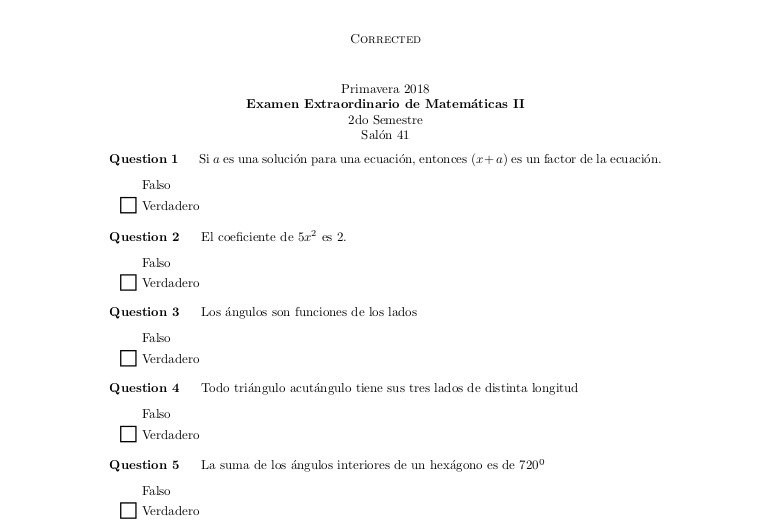
\includegraphics[width=\textwidth]{figures/casillas_sol_mal.jpeg}
                \caption{Solucion generada mal: casillas correctas no aparecen}
                \label{fig:casillasSolMal}
            \end{figure}
            \item generar al menos una versión (usar shuffle para las casillas) \\
            2 versiones distintas con alumnos.csv \\
            ¿cómo activo el shuffle? *
            \item ¿distintas formas de rellenar casillas?
            \item rellenar las casillas de distintas formas y corregir
        \end{itemize}
        \item Shuffle
        \begin{itemize}
            \item La opción shufflechoices está desactivada por defecto, al activar produce un error al faltar el parámetro 'childrenselector' en la llamada a TexSurgery.shuffle(), como se puede observar en la figura \ref{fig:errorShufle}
            \begin{figure}
                \centering
                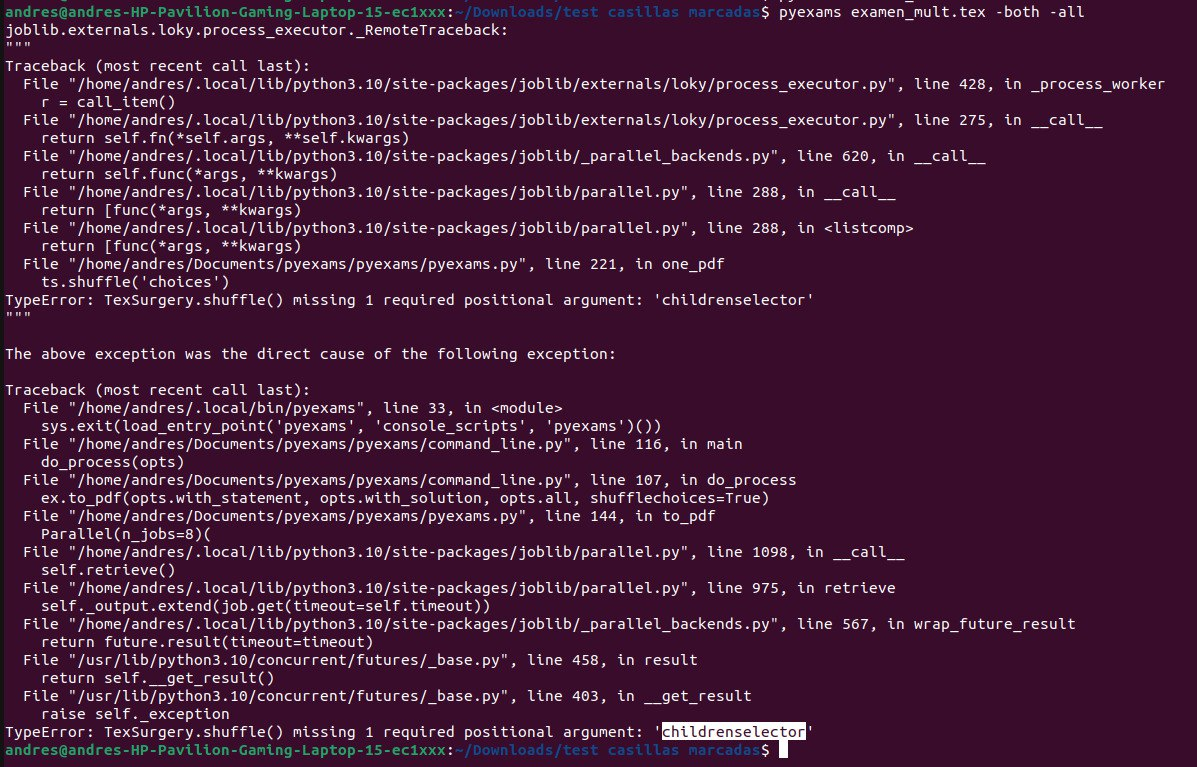
\includegraphics[width=\textwidth]{figures/error_shuffle.jpeg}
                \caption{Error al activar la opción de shuffle}
                \label{fig:errorShufle}
            \end{figure}
        \end{itemize}
        \item Añadir función QR:
        \begin{itemize}
            \item nueva branch en pyexams
            \item guardar info de examen, variante y pagina ¿cómo obtener el numero de pagina?
            el comando \textbackslash{}thepage
            \item la posición debería ser fija si se va a utilizar en reconocimiento de posición/inclinación ¿en el pie de pagina?\\
            pie de pagina: probado librería \textit{fancyhdr}, al meter en un fichero \LaTeX de pyexams no lo genera, ¿AMC se lo carga?\\
            marca de agua: librerías xwatermark, no consigo que compile, y draftwatermark, genera el qr correctamente en cada pagina\\
            \item probar en latex el código para generar qr's, figura \ref{fig:watermark_qr_test}
            \begin{figure}
                \centering
                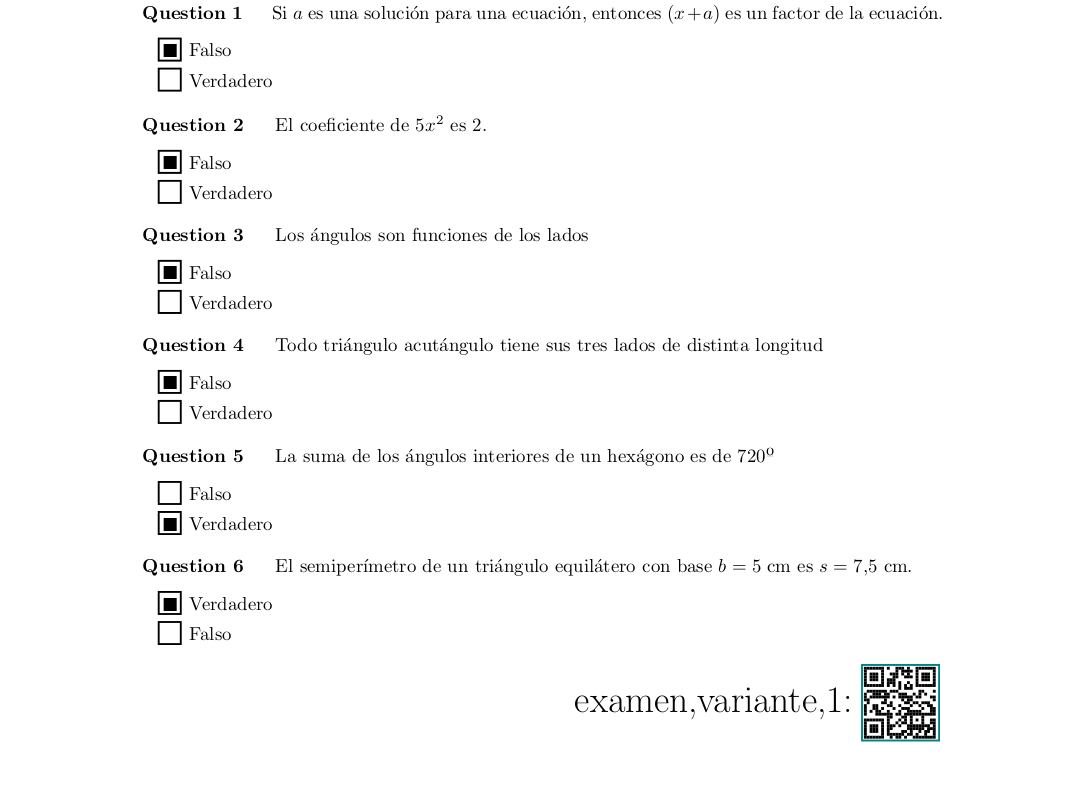
\includegraphics[width=\textwidth]{figures/watermark_qr_test.png}
                \caption{Generación del código QR y texto en claro}
                \label{fig:watermark_qr_test}
            \end{figure}
            \item añadir a pyexams una función que cambie los comandos \textbackslash{}QR por el codigo probado
            \item añadido a la rama "scan" de pyexams en el commit \href{https://framagit.org/pang/pyexams/-/commit/7a32d1f2a68f441a0100cf344400e2952eedd6d1}{"Added function to insert qr codes with the exam id, variant id and page"}: 
            \begin{itemize}
                \item Función qr(tex\_in, exam\_id, variant\_id, watermark\_params):\\
                Parámetros:\\
                \ \ \ \ tex\_in: texto del fichero tex tras procesar con code\_surgery\\
                \ \ \ \ exam\_id: nombre del fichero tex a procesar, identificador del examen\\
                \ \ \ \ variant\_id: id de estudiante, de students.csv, identificador de variante de examen\\
                \ \ \ \ watermark\_params: parámentros para generar la marca de agua (escala, ángulo de giro, color, posición base, y tamaño), con valores por defecto.\\
                Ejecución:\\
                \ \ \ \ Genera un string con el codigo latex que genera un QR con exam\_id, variant\_id y el número de página como una marca de agua con las características indicadas en watermark\_params.\\
                \ \ \ \ Si encuentra el código "\textbackslash{}\textbackslash{}QR" en tex\_in, lo reemplaza por el string mencionado.\\
                \ \ \ \ Devuelve en tex\_out el texto, modificado o no
                \item dentro de la función one\_pdf, que genera un pdf de enunciado/solución para un alumno, y tras procesar el fichero tex con code\_surgery, llama a la función qr pasándole el código tex, el nombre del fichero tex y el id del alumno.
            \end{itemize}
        \end{itemize}
        \item Añadir función de escanear exámenes, partes:
        \begin{itemize}
            \item DETECT: Generar json's al crear enunciados y soluciones
            \item ANALYSE: Añadir función -scan : analizar examenes escaneados/rellenados 
            \item MATCH: corregir los examenes con los json ya generados
        \end{itemize}
        TODO:
        \begin{itemize}
            \item crear branch en pyexams
            \item DETECT: Añadir funciones detect\_statement y detect\_solution a pyexams: reciben el fichero enunciado/solución y crean el json correspondiente
            \item DETECT: Llamar a las funciones detect\_X después de crear los pdf's correspondientes dentro de pyexams
            \item dependencias de las nuevas funciones: PyPDF2 modificado, pdf2image, OpenCV (cv2 en python, existen 4 paquetes distintos en pip, uso opencv-python)
            \item ANALYSE: añadir función scan "pyexams -scan file"
            \item ANALYSE: intentar extraer las casillas con pyPDF2 (rellenado) antes de hacerlo con OpenCV (escaneado)
            \item ANALYSE: (escaneado) leer el QR \\
            no está detectando correctamente el QR, dependiendo del dpi del png detecta los puntos o no, pero no lo decodifica en ningun caso \\
            + mejorar la imagen antes de buscar el QR \\
            + ¿cómo funciona qr\_detect de OpenCV? \\
            Conseguido reconocer los 6 qrs de los examenes de prueba, con el siguiente procesamiento: \\
            Umbralizado la imagen con valor umbral 120 \\
            Aislado los píxeles negros de la imagen \href{https://stackoverflow.com/questions/42592234/python-opencv-morphologyex-remove-specific-color}{(eliminar un color especifico)} \\
            Suavizado (Gaussian blur (3, 3)) y agudizado (sharpen ([-1,-1,-1],[-1,9,-1],[-1,-1,-1])) la imagen sucesivamente \\
            Buscado y decodificado el codigo qr con QRCodeDetector de OpenCV\\
            Detecta correctamente los qrs. Figura \ref{fig:process_qr1}: procesamiento de la imagen para decodificar el QR paso a paso, figura \ref{fig:test_qrs}: QRs recortados tras procesar
            \begin{figure}
                \centering
                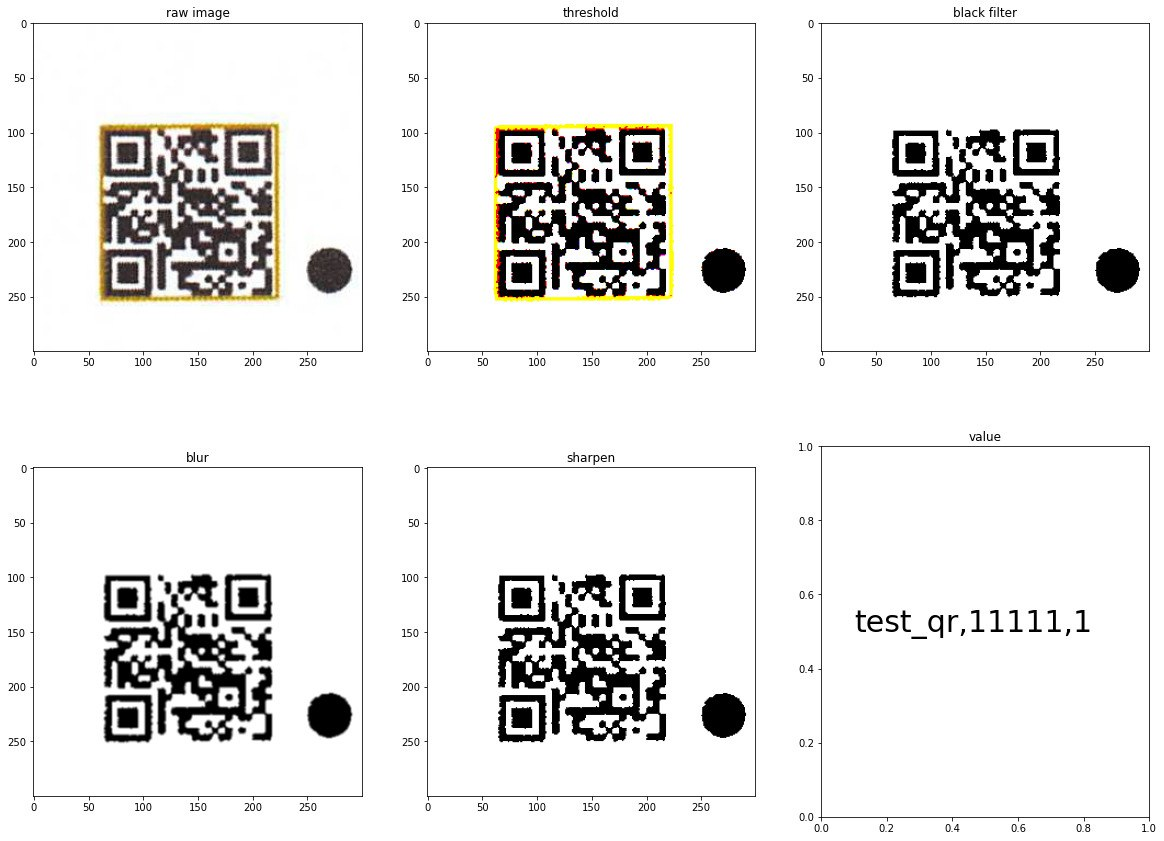
\includegraphics[width=\textwidth]{figures/process_qr1.png}
                \caption{Procesamiento del QR paso a paso}
                \label{fig:process_qr1}
            \end{figure}
            \begin{figure}
                \centering
                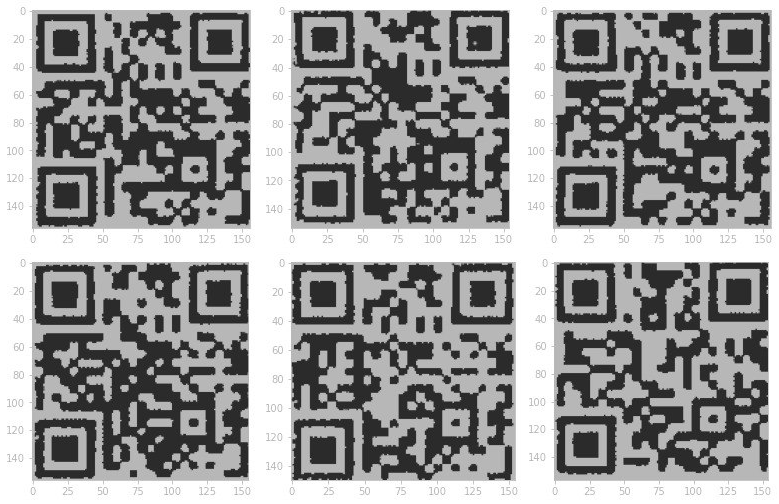
\includegraphics[width=\textwidth]{figures/test_qrs.png}
                \caption{Códigos QR del examen de prueba}
                \label{fig:test_qrs}
            \end{figure}
            \item ANALYSE: (escaneado) extraer las casillas \\
            el tamaño de la imagen depende del dpi, parametrizar el tamaño mínimo de linea para detectar las casillas (dpi: 250 , min\_lin: 35 -> min\_lin: dpi * 0.14) \\
            la función de OpenCV detecta rectángulos con lados mayores al mínimo, hay que identificar cuales de estos rectángulos son casillas y descartar los que no lo son:
            \begin{itemize}
                \item cuadros de texto: tendrán un tamaño mayor al de las casillas, descartar si uno de los lados es mayor al 150\% del mínimo
                \item cuadrados de AMC: están en el cabecero, descartar si la coordenada 'y' es menor al 10\% del alto del documento (obtener el alto del documento a partir del dpi, o del min\_lin: alto = ~11.6 * dpi, ~82.8 * min\_lin )
                \item puntos del QR : sus coordenadas se corresponden a las coordenadas del QR, descartar si se encuentran en un rango basado en las coordenadas del QR
            \end{itemize}
            La función connectedComponentsWithStats() tiene problemas para reconocer casillas marcadas rellenadas de forma manual, cambiado a la función findContours(), que encuentra los contornos de las casillas (ejemplo: \href{https://stackoverflow.com/questions/55169645/square-detection-in-image}{'square detection in image'}). \\
            La función tiene problemas para detectar casillas con bordes muy finos, hay que hacer un pre-procesar la imagen: pasar blanco y negro, suavizar (blur), agudizar (sharpen) y umbral-izar \href{https://docs.opencv.org/4.x/d7/d4d/tutorial_py_thresholding.html}{(threshold de Otsu)}
            \item ANALYSE: (escaneado) identificar si las casillas están marcadas \\
            Extraer el interior de la casilla de sus coordenadas y la imagen binarizada \\
            Ignorar los píxeles cercanos al borde \\
            Si el valor del píxel es mayor a un umbral, sumar uno a un contador, para todos los píxeles \\
            Si el contador es mayor al 10\% del área del interior de la casilla considerar que está marcada
        \end{itemize}
        \item Corregir orientación
        \begin{itemize}
            \item Detectar los círculos de las esquinas (Auto Multiple Choice, \href{https://dl.ucsc.cmb.ac.lk/jspui/bitstream/123456789/4522/1/2013\%20MCS\%20082.pdf}{J. M. M. S Kularathna})
        \end{itemize}
    \end{enumerate}
    \begin{itemize}
        \item Hecho:
        \begin{itemize}
            \item Añadido la función \textbackslash{}QR a pyexams: detecta '\textbackslash{}QR' en los ficheros \LaTeX y lo reemplaza por código que genera un QR con los datos de examen, variante y página en la esquina inferior izquierda de cada página del examen (\href{https://framagit.org/pang/pyexams/-/commit/7a32d1f2a68f441a0100cf344400e2952eedd6d1}{commit 7a32d1f2})
            \item Añadido la función que genera los ficheros JSON con la estructura de los ejercicios y casillas de tanto enunciados como soluciones en la función que genera pdf's de pyexams (\href{https://framagit.org/pang/pyexams/-/commit/caede94e517b2ff57f25c6e9fee53735fe0edae2}{commit caede94e})
            \item Generado un \href{https://github.com/andrsvb/tfg2/blob/e12eb83407ad1875bf4b1cf99487589d2a4c55a8/test%20casillas%20marcadas/test_qr.tex}{fichero \LaTeX} que genera un examen de tres páginas con veinte preguntas de opción múltiple
        \end{itemize}
    \end{itemize}
    \item 10FEB23: Reu en teams
    \begin{itemize}
        \item editar imagen en GIMP para cambiar la perspectiva y probar el reconocimiento del qr.
    \end{itemize}
    \item 10FEB-24FEB23
    \begin{itemize}
        \item Mejorado el preprocesamiento de imagen en la detección de casillas. Inicialmente (figura \ref{fig:detect_boxes_old}), pasaba la imagen a blanco y negro y la umbralizaba. Tras los cambios (figura \ref{fig:detect_boxes_ccws}), la pasa a blanco y negro, suaviza, agudiza y ubraliza con umbral de Otsu. Esto ayuda a detectar las lineas que forman las casillas
        \begin{figure}
            \centering
            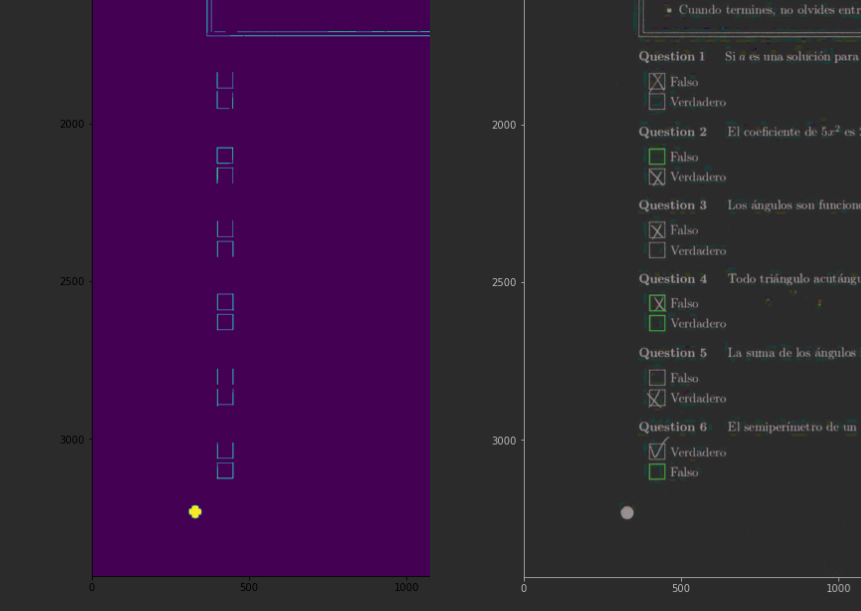
\includegraphics[width=0.8\textwidth]{figures/detect_boxes_old.png}
            \caption{Preprocesamiento inicial}
            \label{fig:detect_boxes_old}
        \end{figure}
        \begin{figure}
            \centering
            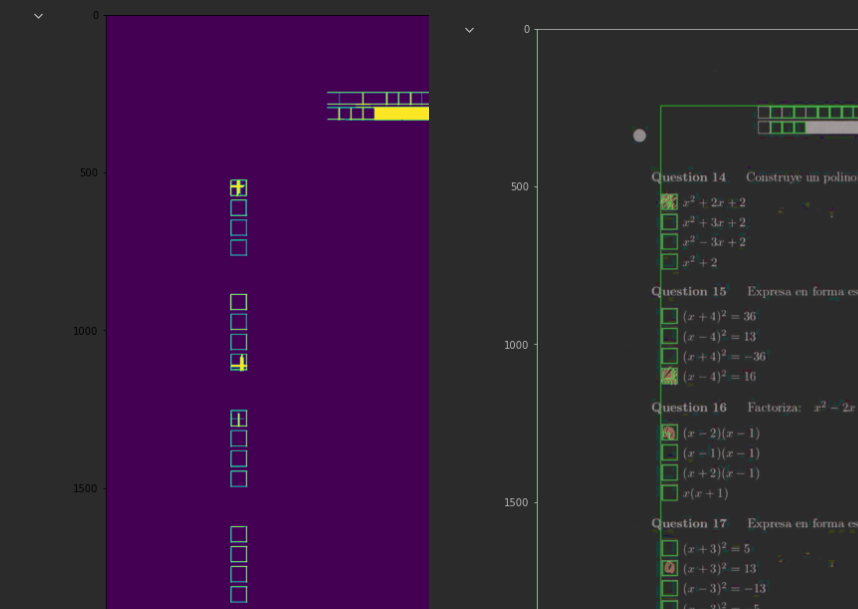
\includegraphics[width=0.8\textwidth]{figures/detect_boxes_ccws.png}
            \caption{Preprocesamiento final}
            \label{fig:detect_boxes_ccws}
        \end{figure}
        \item Cambiado la función que detecta las formas de las casillas. Antes utilizaba connectedComponentsWithStats, que dividía casillas marcadas en varios componentes si el relleno era lo suficientemente grande. La función findContours encuentra los contornos externos, y no divide la casilla. Comparación en la figura \ref{fig:ccws_contours}.
        \begin{figure}
                \centering
                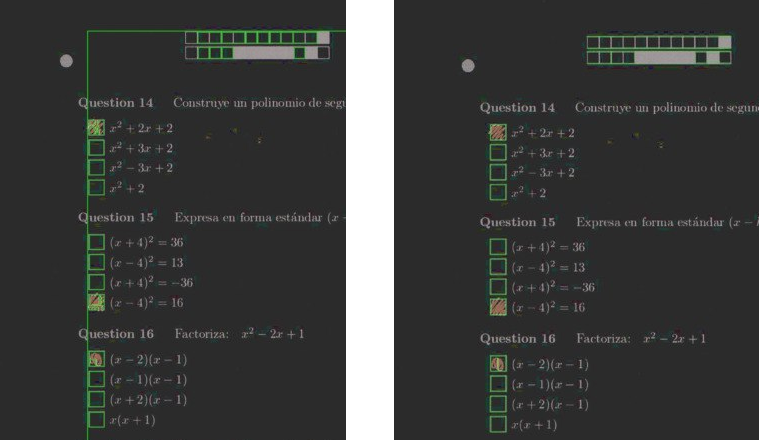
\includegraphics[width=0.9\textwidth]{figures/ccws_contours.png}
                \caption{Componentes conectados - contornos}
                \label{fig:ccws_contours}
        \end{figure}
        \item Clasificación de los contornos detectados. La función detecta varios contornos (figura \ref{fig:detect_boxes_contours}), de los cuales no todos son casillas. Además de casillas, detecta también los cuadros del cabecero de Auto Multiple Choice, cuadros de texto y formas dentro del QR. Descarto estos tipos de contornos según el tipo: cabecero AMC - posición 'y' inferior al 10\% del tamaño de página, cuadros de texto - ancho o largo considerablemente distinto al tamaño de linea definido, y formas del QR - coordenadas interiores a las de los puntos del QR
        \begin{figure}
                \centering
                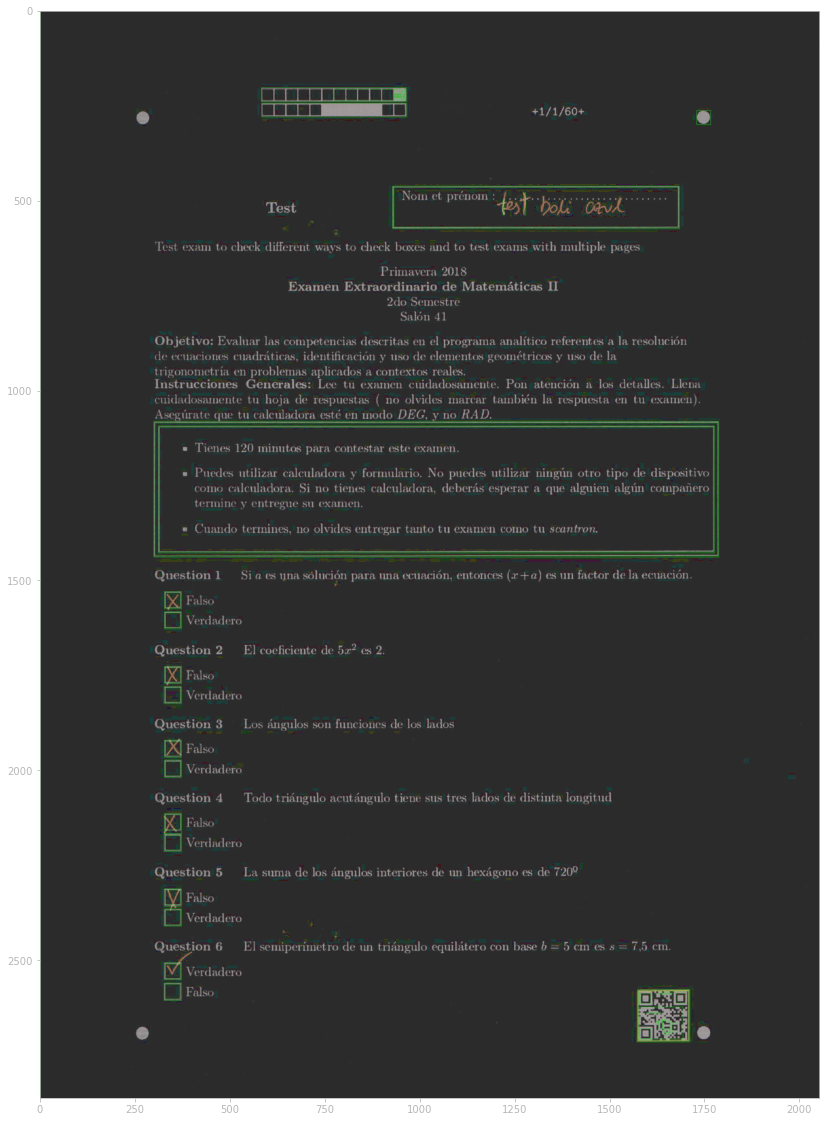
\includegraphics[width=0.9\textwidth]{figures/detect_boxes_contours.png}
                \caption{Identificación de casillas marcadas}
                \label{fig:detect_boxes_contours}
        \end{figure}
        \item Detección de casillas marcadas: extraído los interiores de las casillas a partir de las coordenadas obtenidas de cada contorno, descartado píxeles cercanos al borde para reducir ruido y contado el área rellena. Si este área supera un umbral del tamaño de la casilla, se considera que la casilla está marcada (Ejemplo en la figura \ref{fig:boxes_is_marked}).
        \begin{figure}
                \centering
                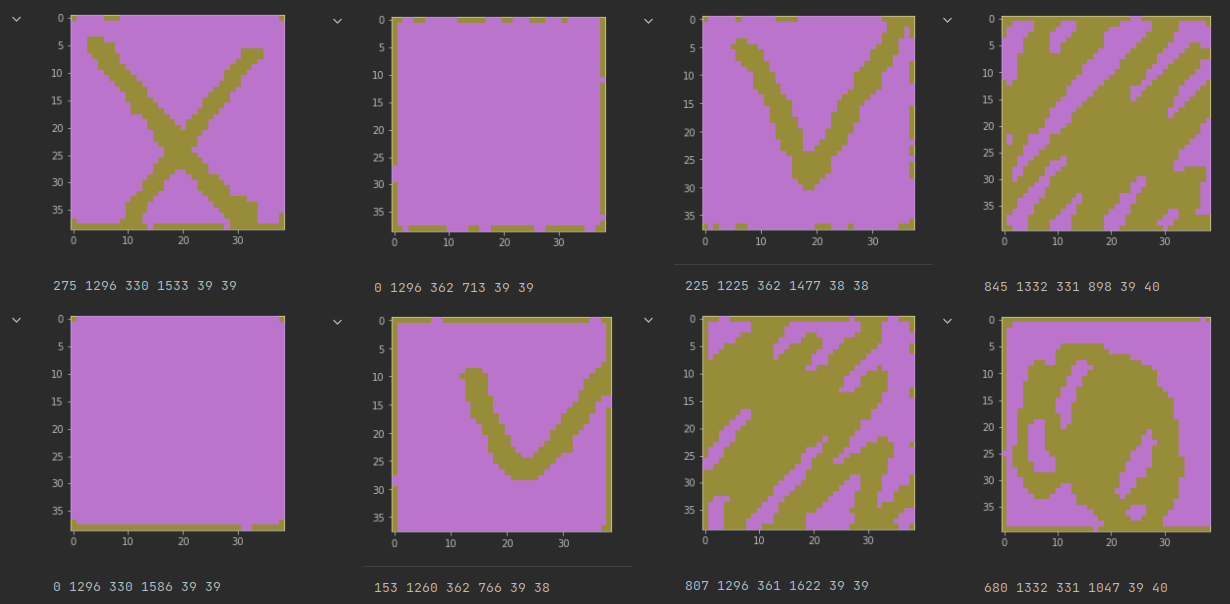
\includegraphics[width=0.9\textwidth]{figures/boxes_is_marked.png}
                \caption{Identificación de casillas marcadas}
                \label{fig:boxes_is_marked}
        \end{figure}
        \item Detección de códigos QR: separado de la detección de casillas y cambiado el preprocesamiento. En este, realiza primero el umbral, extrae los píxeles en negro de la imagen, y por último suaviza y agudiza repetidas veces hasta que encuentra el QR. Este método ha funcionado con los seis codigos de ejemplo, pero no para todas las calidades dpi, siendo poco fiable. (Ejemplo en la figura \ref{fig:detect_qr}).
        \begin{figure}
                \centering
                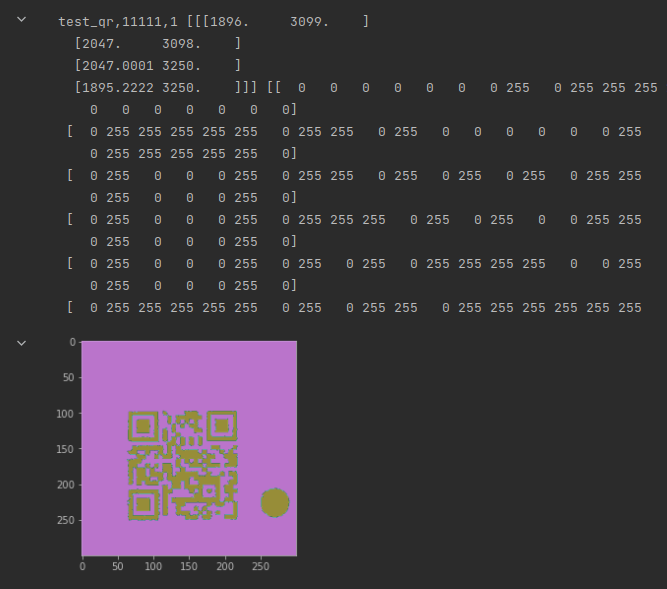
\includegraphics[width=0.9\textwidth]{figures/detect_qr.png}
                \caption{Identificación del código QR}
                \label{fig:detect_qr}
        \end{figure}
    \end{itemize}
    \item 24FEB23: Reu en teams, pang
    \begin{itemize}
        \item Por correos antes de la reunión:\\Resumen de los cambios realizados.\\Definición de dos posibles usos de 'pyexams -scan':
        \begin{itemize}
            \item 'pyexams -scan file.pdf --exam-data DATOS.json'
            \item 'pyexams -scan file.pdf'
        \end{itemize}
        Leer del código QR el identificador de examen y variante.\\
        Si el fichero JSON no se recibe de parámetro, buscar en la ubicación actual o en .pyexams/history o similar.\\
        Leer el fichero JSON, con la información del examen: ejercicios, casillas y coordenadas
        \item Utilizar coordenadas de las casillas (obtenidas con pyPDF2 al generar el pdf, en JSON de enunciado) para identificar los contornos que son casillas. Mejor que descartar los contornos que no pueden ser casillas, reduce error.
        \item Parametrizar el valor umbral de detección de casillas marcadas, manteniendo el valor por defecto.
        \item Guardar el número de página dentro de la información de cada casilla (tanto en detectar como analizar)
        \item Guardar en booleano si la detección del QR ha funcionado
        \item Corrección de exámenes; calificativo para cada respuesta: vacía (ninguna casilla marcada), nula (numero de casillas marcadas distinto a la solución), correcta e incorrecta
        \item Diagrama de flujo de los datos en la funcionalidad 'escanear exámenes'. Figuras \ref{fig:flow_chart_prev}, \ref{fig:flow_chart_post} y \ref{fig:conceptual_layers}: diagrama por pang del flujo antes y después de la funcionalidad, y de las capas conceptuales
        \begin{figure}
                \centering
                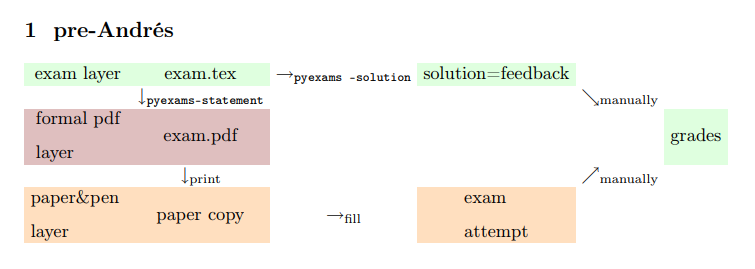
\includegraphics[width=0.9\textwidth]{figures/flow_chart_prev.png}
                \caption{Flujo de la aplicación antes}
                \label{fig:flow_chart_prev}
        \end{figure}
        \begin{figure}
                \centering
                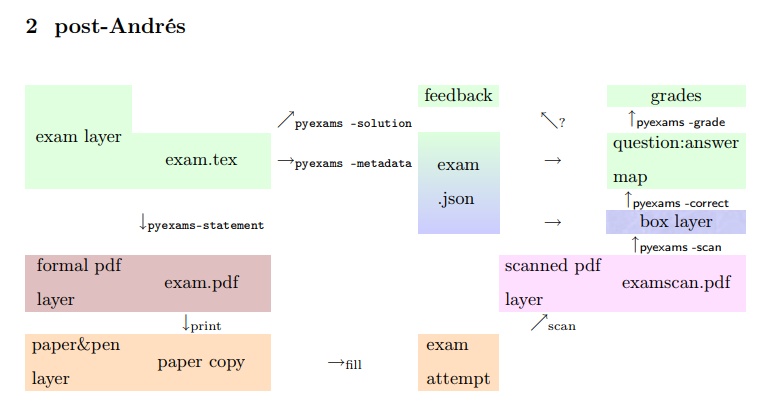
\includegraphics[width=0.9\textwidth]{figures/flow_chart_post.png}
                \caption{Flujo de la aplicación después}
                \label{fig:flow_chart_post}
        \end{figure}
        \begin{figure}
                \centering
                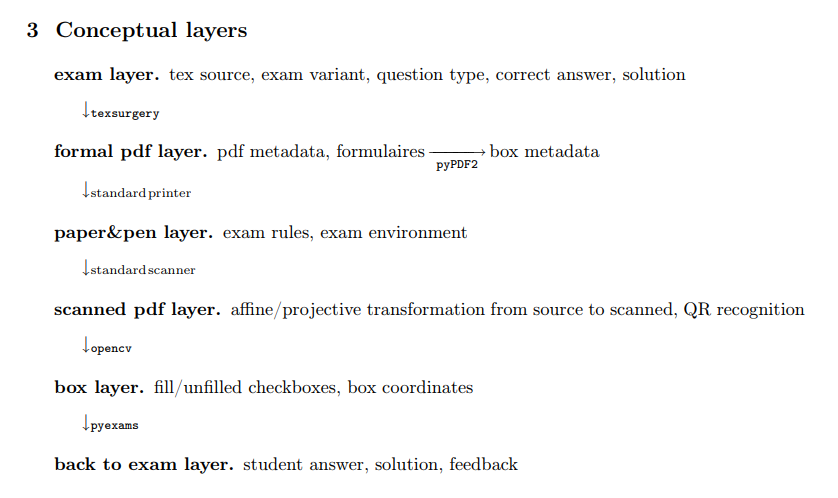
\includegraphics[width=0.9\textwidth]{figures/conceptual_layers.png}
                \caption{Capas conceptuales}
                \label{fig:conceptual_layers}
        \end{figure}
    \end{itemize}
    \item 24FEB23 - 01MAR23
    \begin{itemize}
        \item Añadido parámetro '\textit{validation\_th}' a la función \textit{is\_marked()}, parámetro que corresponde al umbral de área rellenada para considerar la casilla marcada en porcentaje, valor por defecto: 0.1
        \item Guardado el número de página de cada casilla en la función '\textit{analyse}' para examenes escaneados
        \item Guardado el número de página de cada casilla en la función '\textit{detect}' para examenes rellenados. TODO: cambiar también las funciones para enunciados y soluciones generadas
        \item Posible funcionamiento de corregir orientación: con cv2.getStructuringElement, estructura circular y MORPH.OPEN -> extraer los círculos de AMC, obtener coordenadas y 'corregir' la imagen. Para corregir se puede: a) transformar la imagen modificando los pixeles, b) modificar el sistema de coordenadas para transformar las coordenadas en el examen escaneado a coordenadas rectificadas
        \item Detección de casillas. Al tener ya las coordenadas de las casillas en el enunciado, identificar las casillas en los exámenes escaneados buscando solo en las zonas cercanas a dichas coordenadas
        \item ¿Procesar la pagina directamente en vez de guardarla en un png para después leerla?
    \end{itemize}
    \item 01MAR23, Reu en teams: pang, carlos, angel, sandra
    \begin{itemize}
        \item El programa creado se puede adaptar para corregir cualquier examen tipo test, no solo generados con pyexams. Definir este caso de uso alternativo. Posibilidad de crear una librería con esa funcionalidad aparte y que pyexams la llame, por temas de cohesión en los comandos de pyexams.
        \item Pasos a seguir: terminar el código (~1 semana); TODO: limpiar bitacora, ampliar estado cuestión y requisitos; empezar trabajo memoria con Sandra (~4 semanas)
        \item demo grabada para la defensa: grabado los pasos sin voz y explicación en vivo
        \item Función QR no funciona a pang, correos. Fichero sty? Distinta versión python? Función QR sólo funciona con -both -all?
    \end{itemize}
    \item 01MAR23 - 13MAR23
    \begin{itemize}
        \item Añadido función format\_scan que cambia las casillas detectadas al formato json definido
        \item lectura de los json de enunciado y de solución
        \item añadido función grade que compara el json solución con el json enunciado, clasificando cada ejercicio en: empty, null, correct e incorrect
        \item probado la ejecución con los dos exámenes escaneados y dos exámenes mas, rellenados con editor pdf (figura \ref{fig:run_2scan_2filled})
        \begin{figure}
                \centering
                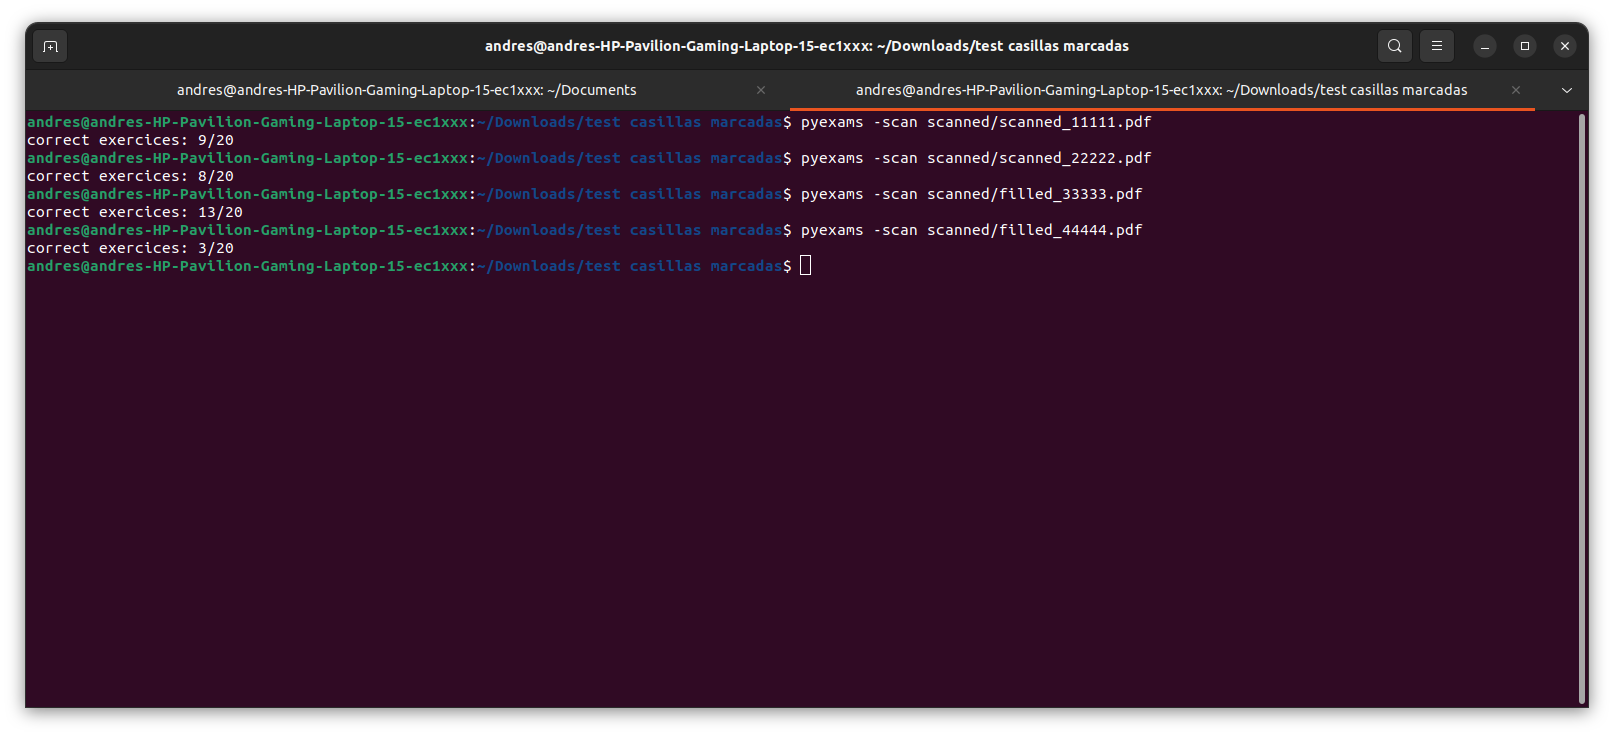
\includegraphics[width=0.9\textwidth]{figures/run_2scan_2filled.png}
                \caption{Ejecución con dos exámenes escaneados y dos rellenados}
                \label{fig:run_2scan_2filled}
        \end{figure}
    \end{itemize}
    \item 13MAR23, Reu en navales: pang
    \begin{itemize}
        \item Identificar qué casilla de OpenCV es qué casilla de pyPDF2 no existe, funciona con fe ciega :) (ambas detectan casillas por el mismo orden de posición, pero en caso de error no funcionaria)
        \item Al tener las coordenadas de los 4 puntos del QR, se puede realizar una transformación (TODO: pang)
        \item probar detección de qrs con  giros de distintos grados
        \item si buscas directamente dentro de un rango de coordenadas donde consideras que están las casillas:
        \begin{itemize}
            \item fiabilidad: ancho, coordenadas, giro (tests con examenes girados)
            \item find contours dentro de un subarray para cada casilla?
        \end{itemize}
        \item comprobar si el parámetro de -scan es un fichero/carpeta, función para corregir carpetas, throw exception si no existe
    \end{itemize}
    \item 13MAR23 - X
    \begin{itemize}
        \item 
        \item Buscado la relación (proporcional al dpi) entre las coordenadas de pyPDF2 y en OpenCV (figura \ref{fig:dpi_transformation})
        \begin{figure}
                \centering
                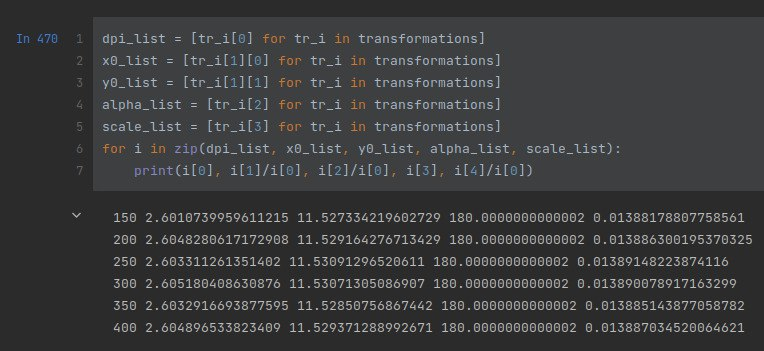
\includegraphics[width=0.9\textwidth]{figures/dpi_transformation.jpeg}
                \caption{Relación entre las coordenadas en pyPDF2 y OpenCV, en función del dpi}
                \label{fig:dpi_transformation}
        \end{figure}
    \end{itemize}
\end{itemize}